\section{总结与使用 \texttt{scikit-learn}}
\label{sec:chapter15}

\subsection{总结}

吴恩达老师的机器学习系列课程到这里就结束了，$40$ 天里，我学到了许多有趣的、极具吸引力的机器学习知识，相信若干年后想起这段时光，仍然会感谢吴恩达老师带我入门了这个领域。

在这门课上，我们学习了以下内容：

\begin{itemize}
    \item 监督学习 Supervised learning
      \begin{itemize}
        \item 线性回归 Linear regression （第 \ref{sec:chapter1},\ref{sec:chapter2},\ref{sec:chapter3} 章）
        \item 逻辑回归 Logistic regression（第 \ref{sec:chapter4},\ref{sec:chapter5},\ref{sec:chapter6} 章）
        \item (BP)神经网络 Neural networks（第 \ref{sec:chapter7},\ref{sec:chapter8} 章）
        \item 支持向量机 Support vector machines（第 \ref{sec:chapter10} 章）
      \end{itemize}
    \item 无监督学习 Unsupervised learning
      \begin{itemize}
        \item K-Means（第 \ref{sec:chapter11} 章）
        \item 主成分分析 Principal component analysis（第 \ref{sec:chapter12} 章）
        \item 异常检测 Anomaly detection（第 \ref{sec:chapter13} 章）
      \end{itemize}
    \item 特殊应用/特殊专题
      \begin{itemize}
        \item 推荐系统 Recommender systems（协同过滤 Collaborative filtering）（第 \ref{sec:chapter14} 章）
        \item 大规模机器学习 Large scale machine learning
      \end{itemize}
    \item 建立机器学习模型时的一些建议
      \begin{itemize}
        \item 方差与偏差 Bias / variance（第 \ref{sec:chapter9} 章）
        \item 正则化 Regularization（第 \ref{sec:chapter5} 章）
        \item 对学习算法的评价：precision, recall, f1 score
        \item 学习曲线 Learning curves（第 \ref{sec:chapter9} 章）
        \item 误差分析 Error analysis
        \item 上界分析 Ceiling analysis
      \end{itemize}
\end{itemize}


\subsection{使用 \texttt{scikit-learn} 进行机器学习}

学习过程中的代码基本都是自己实现的，运行效率和使用容易程度上不敢恭维……现在清楚了原理之后，就可以放心大胆地调包了。

\paragraph{线性回归}

\begin{center}
\begin{lstlisting}[language=Python]
"""
class sklearn.linear_model.LinearRegression(*, fit_intercept=True, 
normalize=False, copy_X=True, n_jobs=None, positive=False)
"""

import numpy as np
import matplotlib.pyplot as plt
from sklearn.linear_model import LinearRegression

data = np.loadtxt('data/ex1data1.txt', delimiter=',')
y = data[:, -1]
X = data[:, :-1]

reg = LinearRegression(normalize=True)
reg.fit(X, y)
print(reg.score(X, y))

ax = plt.subplot(1, 1, 1)
ax.set_xlabel('x')
ax.set_ylabel('y')
ax.set_title('Linear Regression')
ax.plot(X.flatten(), y, 'x', color='red')
ax.plot(X, reg.predict(X))
plt.show()
\end{lstlisting}
\end{center}

\begin{figure}[H]
    \centering
    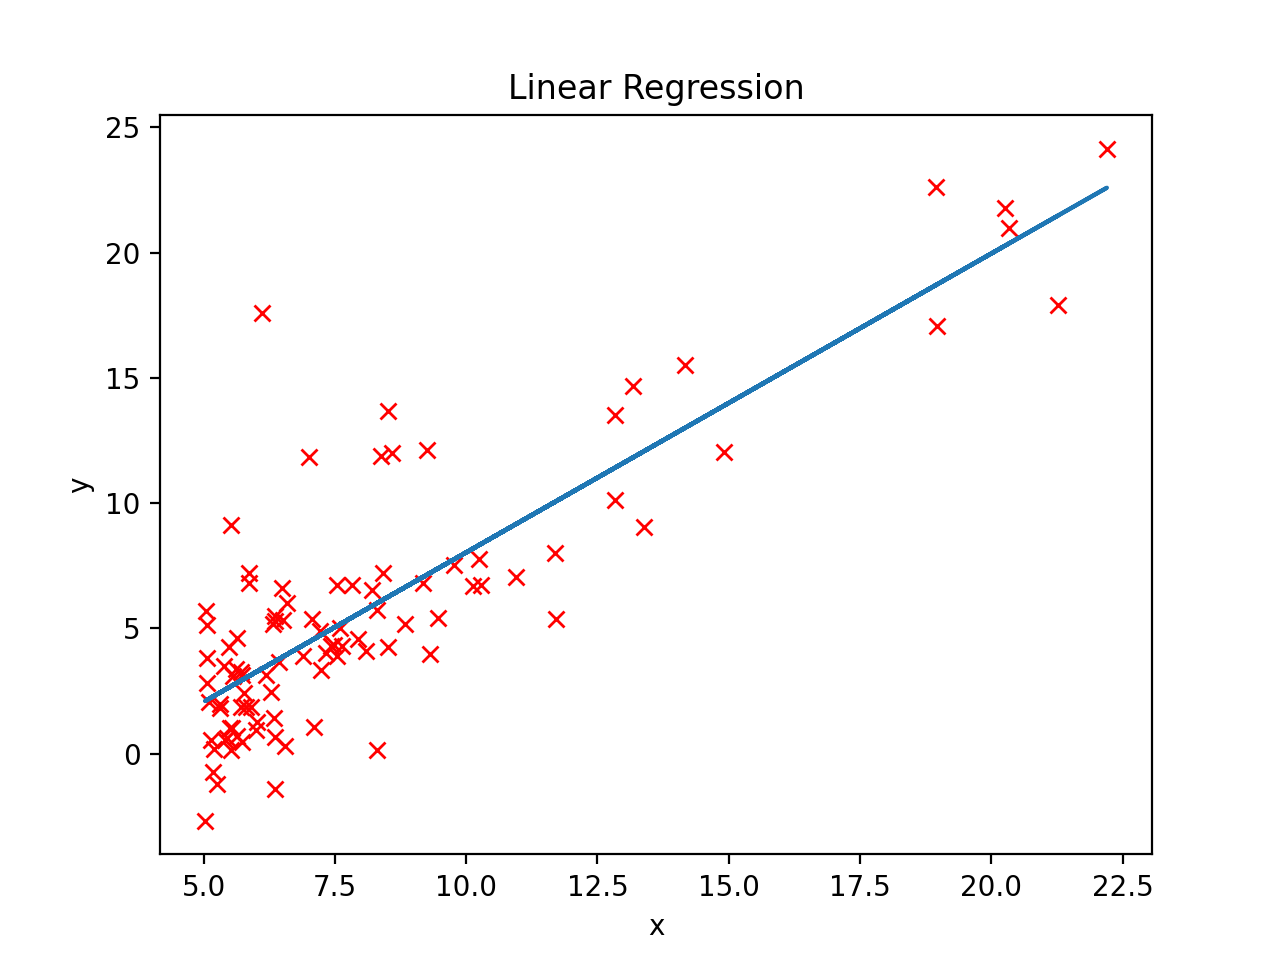
\includegraphics[width=0.5\linewidth]{figs/Chap_15_LinearRegression.png}
\end{figure}

\begin{lstlisting}[language=Python]
"""
class sklearn.linear_model.LinearRegression(*, fit_intercept=True, 
normalize=False, copy_X=True, n_jobs=None, positive=False)
"""

import numpy as np
import matplotlib.pyplot as plt
from sklearn.linear_model import LinearRegression

data = np.loadtxt('data/ex1data2.txt', delimiter=',')
y = data[:, -1]
X = data[:, :-1]

reg = LinearRegression(normalize=True)
reg.fit(X, y)
print(reg.score(X, y))
print(reg.predict(X))
\end{lstlisting}

\paragraph{逻辑回归}

\begin{center}
\begin{lstlisting}[language=Python]
"""
class sklearn.linear_model.LogisticRegression(penalty='l2', *, dual=False, 
tol=0.0001, C=1.0, fit_intercept=True, intercept_scaling=1, 
class_weight=None, random_state=None, solver='lbfgs', max_iter=100, 
multi_class='auto', verbose=0, warm_start=False, n_jobs=None, l1_ratio=None)
"""

import numpy as np
import matplotlib.pyplot as plt
from sklearn.linear_model import LogisticRegression

data = np.loadtxt('data/ex2data1.txt', delimiter=',')
y = data[:, -1]
X = data[:, :-1]

clf = LogisticRegression()
clf.fit(X, y)
print(clf.score(X, y))

ax = plt.subplot(1, 1, 1)
ax.set_xlabel('x1')
ax.set_ylabel('x2')
ax.set_title('Logistic Regression')
ax.plot(X[y==0][:, 0], X[y==0][:, 1], 'x', color='red')
ax.plot(X[y==1][:, 0], X[y==1][:, 1], 'o', color='blue', markerfacecolor='none')
x1, x2 = np.meshgrid(np.linspace(X[:, 0].min(), X[:, 0].max(), 100), 
	np.linspace(X[:, 1].min(), X[:, 1].max(), 100))
ax.contour(x1, x2, 
	clf.predict_proba(np.array([x1, x2]).\
	transpose(2, 1, 0).reshape((10000, 2)))[:, 0].reshape(100, 100), [0.5])
ax.axis('square')

plt.show()
\end{lstlisting}
\end{center}

\begin{figure}[H]
    \centering
    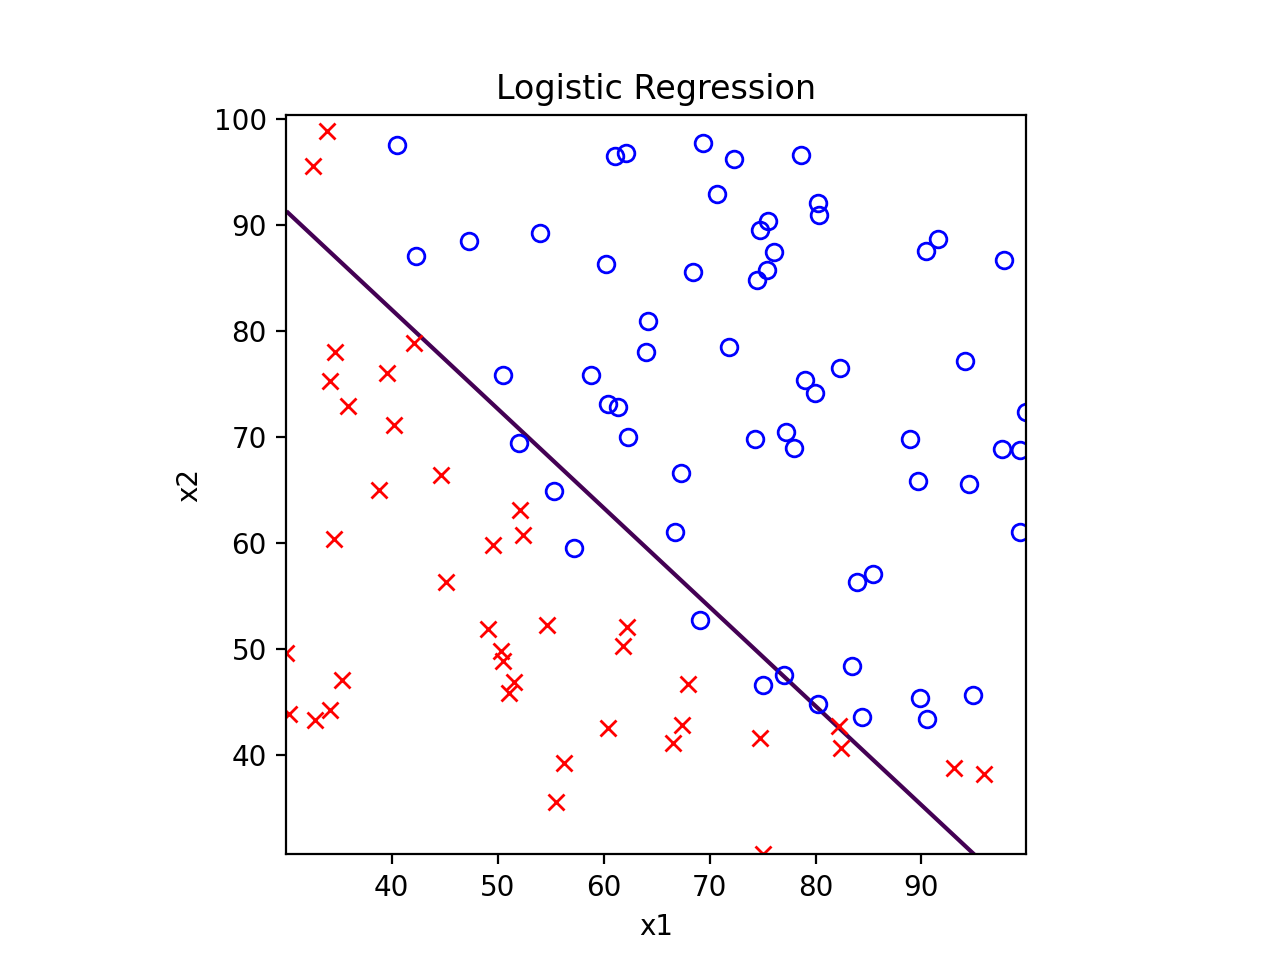
\includegraphics[width=0.5\linewidth]{figs/Chap_15_LogisticRegression.png}
\end{figure}

\begin{lstlisting}[language=Python]
"""
class sklearn.linear_model.LogisticRegression(penalty='l2', *, dual=False, 
tol=0.0001, C=1.0, fit_intercept=True, intercept_scaling=1, 
class_weight=None, random_state=None, solver='lbfgs', max_iter=100, 
multi_class='auto', verbose=0, warm_start=False, n_jobs=None, l1_ratio=None)

class sklearn.preprocessing.PolynomialFeatures(degree=2, *, 
interaction_only=False, include_bias=True, order='C')
"""

import numpy as np
import matplotlib.pyplot as plt
from sklearn.linear_model import LogisticRegression
from sklearn.linear_model import LogisticRegressionCV
from sklearn.preprocessing import PolynomialFeatures

data = np.loadtxt('data/ex2data2.txt', delimiter=',')
y = data[:, -1]
X = data[:, :-1]
poly = PolynomialFeatures(degree=5)
newX = poly.fit_transform(X)

fig, ax = plt.subplots(1, 4)
fig.suptitle('Logistic Regression')
Cs = [0.01, 1, 300, -1]
for i in range(4):
	C = Cs[i]
	if i < 3:
		clf = LogisticRegression(C=C, max_iter=1000)
	else:
		clf = LogisticRegressionCV(max_iter=1000)
	clf.fit(newX, y)
	print(clf.score(newX, y))

	if i < 3:
		ax[i].set_title('C={0}'.format(C))
	else:
		ax[i].set_title('LogisticRegressionCV')
	ax[i].plot(X[y==0][:, 0], X[y==0][:, 1], 'x', color='red')
	ax[i].plot(X[y==1][:, 0], X[y==1][:, 1], 'o', color='blue', markerfacecolor='none')
	x1, x2 = np.meshgrid(np.linspace(X[:, 0].min(), X[:, 0].max(), 100), 
		np.linspace(X[:, 1].min(), X[:, 1].max(), 100))
	ax[i].contour(x1, x2, clf.predict_proba(
		poly.transform(np.array([x1, x2]).transpose(1, 2, 0).reshape((10000, 2)))
		)[:, 0].reshape(100, 100), [0.5])
	ax[i].axis('square')

plt.show()
\end{lstlisting}

\begin{figure}[H]
    \centering
    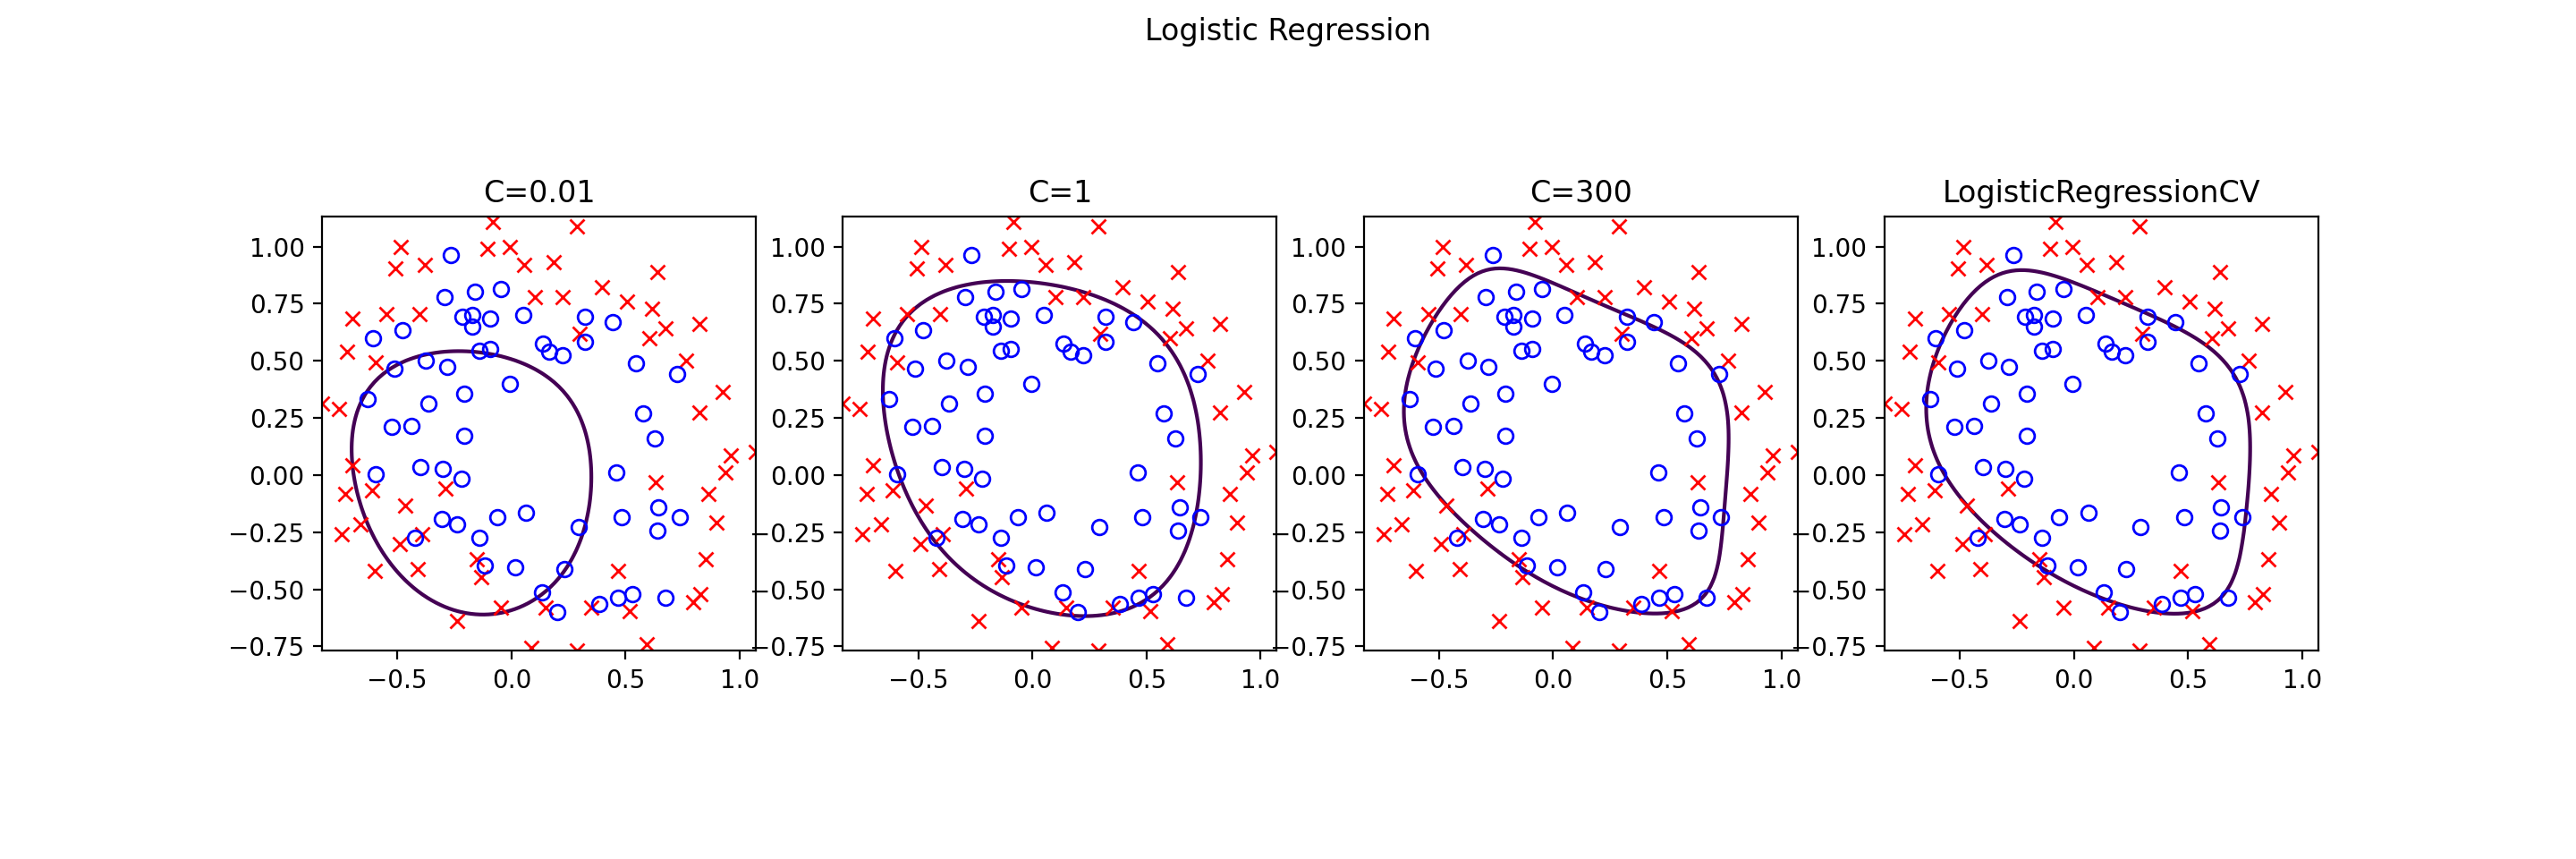
\includegraphics[width=\linewidth]{figs/Chap_15_LogisticRegression2.png}
\end{figure}

\paragraph{多项式回归}

\begin{center}
\begin{lstlisting}[language=Python]
"""
class sklearn.linear_model.Ridge(alpha=1.0, *, fit_intercept=True, normalize=False, 
copy_X=True, max_iter=None, tol=0.001, solver='auto', random_state=None)

class sklearn.preprocessing.PolynomialFeatures(degree=2, *, 
interaction_only=False, include_bias=True, order='C')
"""

import numpy as np
import matplotlib.pyplot as plt
from scipy.io import loadmat
from sklearn.linear_model import Ridge
from sklearn.linear_model import RidgeCV
from sklearn.preprocessing import PolynomialFeatures

data = loadmat('data/ex5data1.mat')
X = data['X']
y = data['y']
poly = PolynomialFeatures(degree=8)
newX = poly.fit_transform(X)

alphas = [0, 0.05, 10, -1]
fig, ax = plt.subplots(1, 4)
fig.suptitle('Polynomial Regression')
for i in range(4):
	alpha = alphas[i]
	if alpha == -1:
		reg = RidgeCV(normalize=True)
	else:
		reg = Ridge(alpha=alpha, normalize=True)
	reg.fit(newX, y)
	print(reg.score(newX, y))

	if alpha >= 0:
		ax[i].set_title('alpha={0}'.format(alpha))
	else:
		ax[i].set_title('RidgeCV')
	ax[i].plot(X.flatten(), y, 'x', color='red')
	ax[i].plot(np.linspace(X.min()-5, X.max()+5, 100), \
		reg.predict(poly.transform( np.linspace(X.min()-5, X.max()+5, 100).reshape((100, 1))) ))

plt.show()
\end{lstlisting}
\end{center}

\begin{figure}[H]
    \centering
    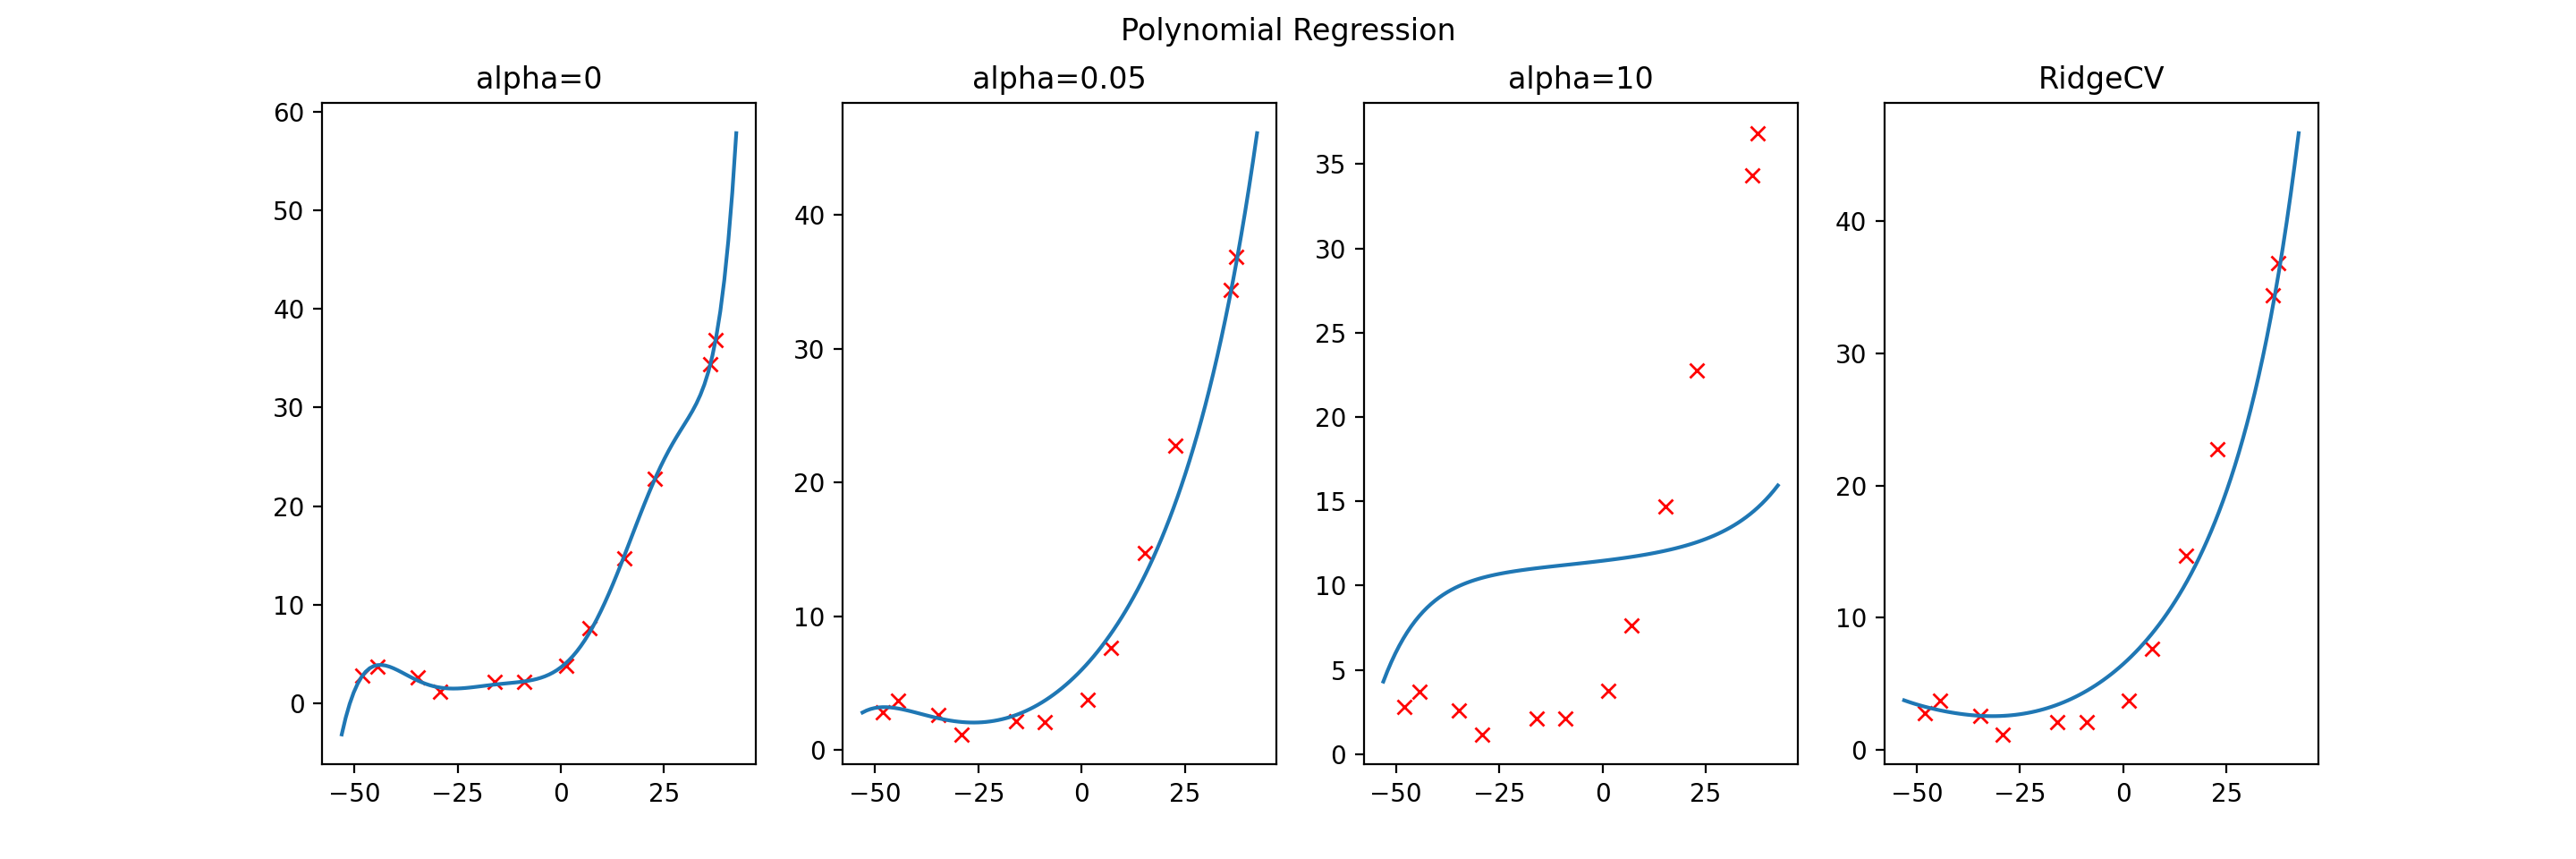
\includegraphics[width=\linewidth]{figs/Chap_15_PolynomialRegression.png}
\end{figure}


\paragraph{BP 神经网络}

\begin{center}
\begin{lstlisting}[language=Python]
"""
class sklearn.neural_network.MLPClassifier(hidden_layer_sizes=100, activation='relu', *, 
solver='adam', alpha=0.0001, batch_size='auto', learning_rate='constant', 
learning_rate_init=0.001, power_t=0.5, max_iter=200, shuffle=True, random_state=None, 
tol=0.0001, verbose=False, warm_start=False, momentum=0.9, nesterovs_momentum=True, 
early_stopping=False, validation_fraction=0.1, beta_1=0.9, beta_2=0.999, epsilon=1e-08, 
n_iter_no_change=10, max_fun=15000)
"""

import numpy as np
from scipy.io import loadmat
from sklearn.model_selection import train_test_split
from sklearn.neural_network import MLPClassifier

data = loadmat('data/ex4data1.mat')
X = data['X']
m = X.shape[0]
X = np.transpose(X.reshape(m, 20, 20), [0, 2, 1]).reshape(m, 400)
y = data['y']
y[y==10] = 0
y = y.flatten()
X_train, X_test, y_train, y_test = train_test_split(X, y, train_size = 0.8)

clf = MLPClassifier(hidden_layer_sizes=(25,), 
					random_state=True, 
					max_iter=1000)
clf.fit(X_train, y_train)
print(clf.score(X_test, y_test))
\end{lstlisting}
\end{center}

\paragraph{支持向量机}

\begin{center}
\begin{lstlisting}[language=Python]
"""
class sklearn.svm.LinearSVC(penalty='l2', loss='squared_hinge', *, dual=True, 
tol=0.0001, C=1.0, multi_class='ovr', fit_intercept=True, intercept_scaling=1, 
class_weight=None, verbose=0, random_state=None, max_iter=1000)
"""

import numpy as np
import matplotlib.pyplot as plt
from scipy.io import loadmat
from sklearn.svm import LinearSVC

data = loadmat('data/ex6data1.mat')
X = data['X']
y = data['y'].flatten()

Cs = [1, 100]
fig, ax = plt.subplots(1, 2)
fig.suptitle('LinearSVC')
x1, x2 = np.meshgrid(np.linspace(X[:, 0].min()-0.5, X[:, 0].max()+0.5, 100), 
	np.linspace(X[:, 1].min()-0.5, X[:, 1].max()+0.5, 100))
for i in range(2):
	C = Cs[i]
	clf = LinearSVC(C=C)
	clf.fit(X, y)
	print(clf.predict(X[:10]))

	ax[i].plot(X[y==0][:, 0], X[y==0][:, 1], 'x', color='red')
	ax[i].plot(X[y==1][:, 0], X[y==1][:, 1], 'o', color='blue')
	ax[i].contour(x1, x2, clf.decision_function(
		np.array([x1, x2]).transpose(1, 2, 0).reshape(10000, 2)
		).reshape(100, 100), [0])
	ax[i].set_xlabel('x1')
	ax[i].set_ylabel('x2')
	ax[i].set_title('C={0}'.format(C))
	ax[i].axis('square')

plt.show()
\end{lstlisting}
\end{center}

\begin{figure}[H]
    \centering
    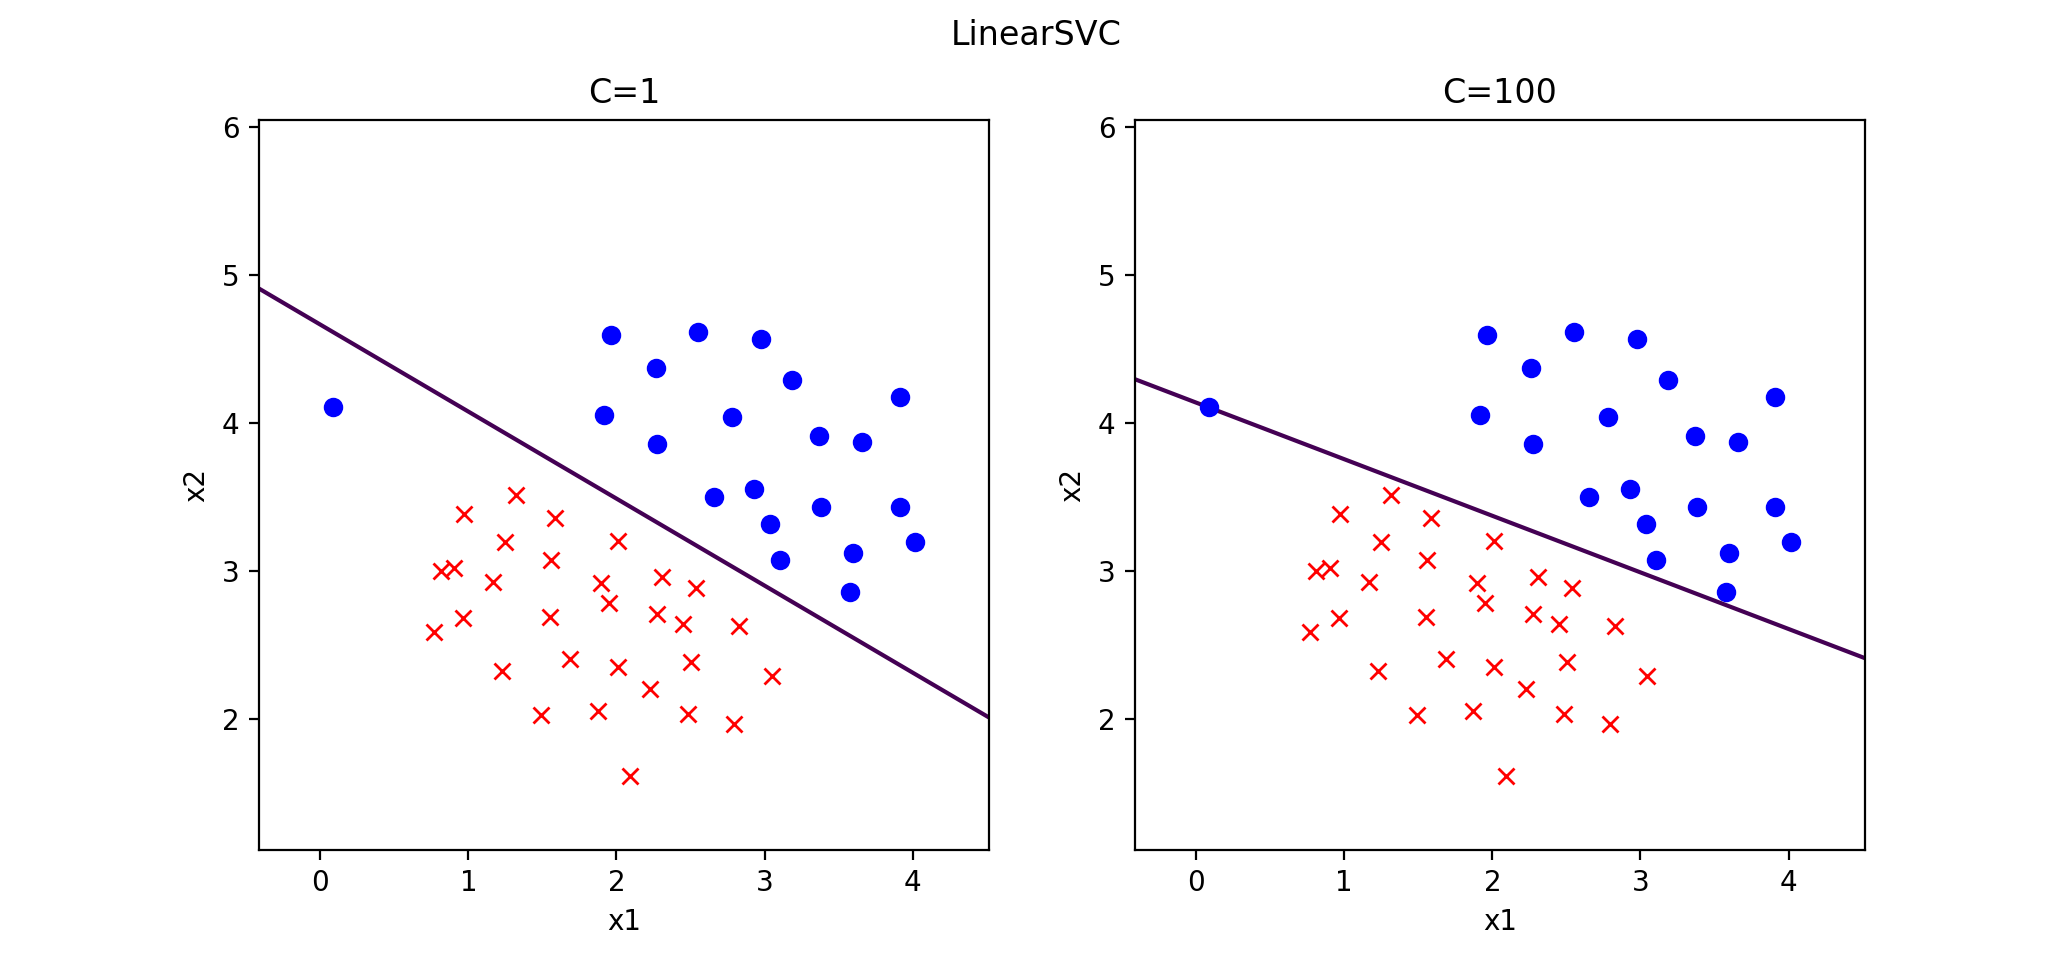
\includegraphics[width=\linewidth]{figs/Chap_15_LinearSVC.png}
\end{figure}

\begin{lstlisting}[language=Python]
"""
class sklearn.svm.SVC(*, C=1.0, kernel='rbf', degree=3, gamma='scale', 
coef0=0.0, shrinking=True, probability=False, tol=0.001, cache_size=200, 
class_weight=None, verbose=False, max_iter=- 1, decision_function_shape='ovr', 
break_ties=False, random_state=None)
"""

import numpy as np
import matplotlib.pyplot as plt
from scipy.io import loadmat
from sklearn.svm import SVC

data = loadmat('data/ex6data2.mat')
X = data['X']
y = data['y'].flatten()

Cs, gammas = [1, 100], [1, 10, 30]
fig, ax = plt.subplots(2, 3)
fig.suptitle('SVC')
x1, x2 = np.meshgrid(np.linspace(X[:, 0].min(), X[:, 0].max(), 100), 
	np.linspace(X[:, 1].min(), X[:, 1].max(), 100))
for i in range(2):
	for j in range(3):
		C, gamma = Cs[i], gammas[j]
		clf = SVC(C=C, kernel='rbf', probability=True, gamma=gamma)
		clf.fit(X, y)

		ax[i][j].plot(X[y==0][:, 0], X[y==0][:, 1], 'x', color='red', alpha=0.5)
		ax[i][j].plot(X[y==1][:, 0], X[y==1][:, 1], 'o', color='blue', markerfacecolor='none', alpha=0.5)
		ax[i][j].contour(x1, x2, clf.decision_function(
			np.array([x1, x2]).transpose(1, 2, 0).reshape(10000, 2)
			).reshape(100, 100), [0])
		ax[i][j].set_title('C={0}, gamma={1}'.format(C, gamma))

plt.show()
\end{lstlisting}

\begin{figure}[H]
    \centering
    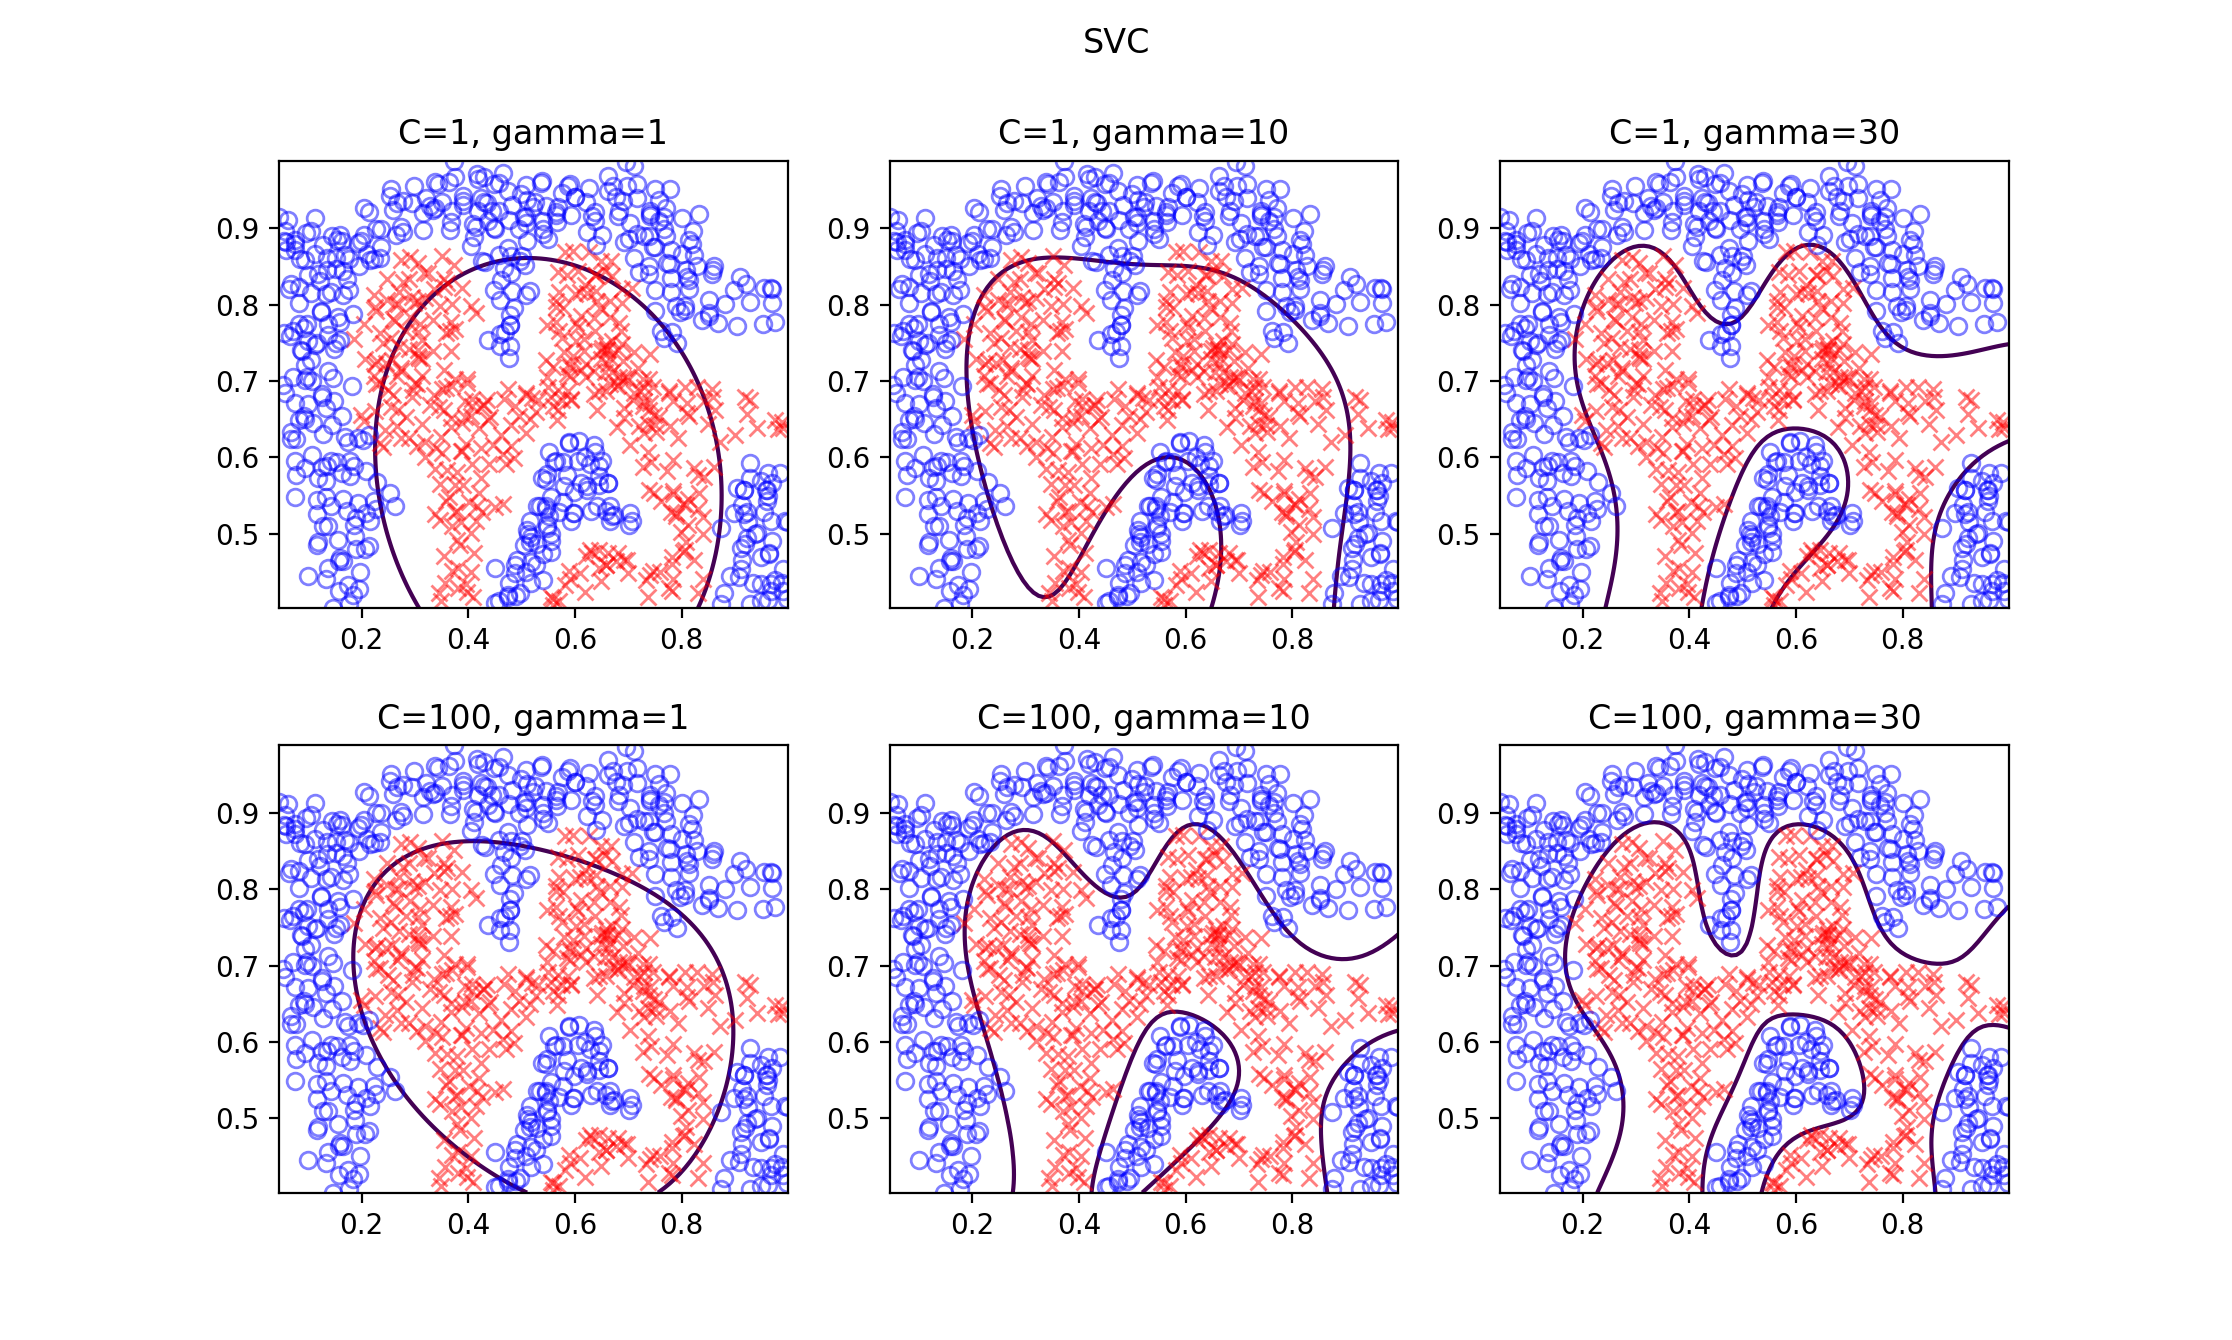
\includegraphics[width=\linewidth]{figs/Chap_15_SVC.png}
\end{figure}


\paragraph{K-Means}

\begin{center}
\begin{lstlisting}[language=Python]
"""
class sklearn.cluster.KMeans(n_clusters=8, *, init='k-means++', n_init=10, 
max_iter=300, tol=0.0001, precompute_distances='deprecated', verbose=0, 
random_state=None, copy_x=True, n_jobs='deprecated', algorithm='auto')
"""

import numpy as np
from scipy.io import loadmat
import matplotlib.pyplot as plt
from sklearn.cluster import KMeans

data = loadmat('data/ex7data2.mat')
X = data['X']

clt = KMeans(n_clusters=3)
belong = clt.fit_predict(X)

ax = plt.subplot(1, 1, 1)
ax.plot(X[belong==0][:, 0], X[belong==0][:, 1], 'o', color='blue', markerfacecolor='none')
ax.plot(X[belong==1][:, 0], X[belong==1][:, 1], 'o', color='red', markerfacecolor='none')
ax.plot(X[belong==2][:, 0], X[belong==2][:, 1], 'o', color='green', markerfacecolor='none')
ax.set_title('KMeans')
plt.show()
\end{lstlisting}
\end{center}

\begin{figure}[H]
    \centering
    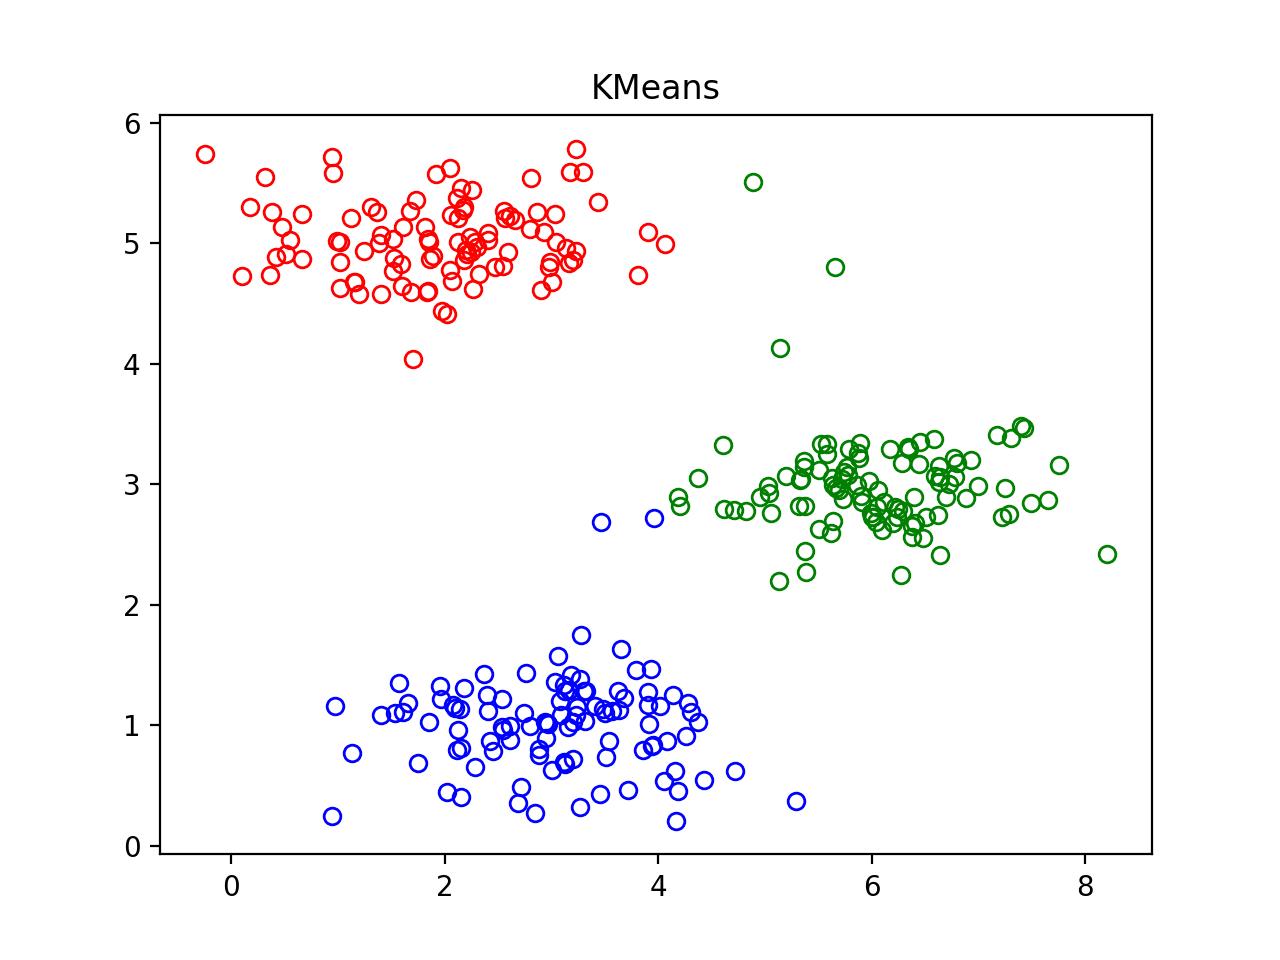
\includegraphics[width=0.5\linewidth]{figs/Chap_15_KMeans.png}
\end{figure}

\paragraph{主成分分析}

\begin{center}
\begin{lstlisting}[language=Python]
"""
class sklearn.decomposition.PCA(n_components=None, *, copy=True, whiten=False, 
svd_solver='auto', tol=0.0, iterated_power='auto', random_state=None)
"""

import numpy as np
from scipy.io import loadmat
import matplotlib.pyplot as plt
from sklearn.decomposition import PCA

data = loadmat('data/ex7data1.mat')
X = data['X']

pca = PCA(n_components=1)
pca.fit(X)
redX = pca.transform(X) # reduced X
recX = pca.inverse_transform(redX) # recovered X

ax = plt.subplot(1, 1, 1)
ax.plot(X[:, 0], X[:, 1], 'o', color='black', markerfacecolor='none')
ax.plot(recX[:, 0], recX[:, 1], 'o', color='red', markerfacecolor='none')
ax.set_title('PCA')
ax.axis('square')
plt.show()
\end{lstlisting}
\end{center}

\begin{figure}[H]
    \centering
    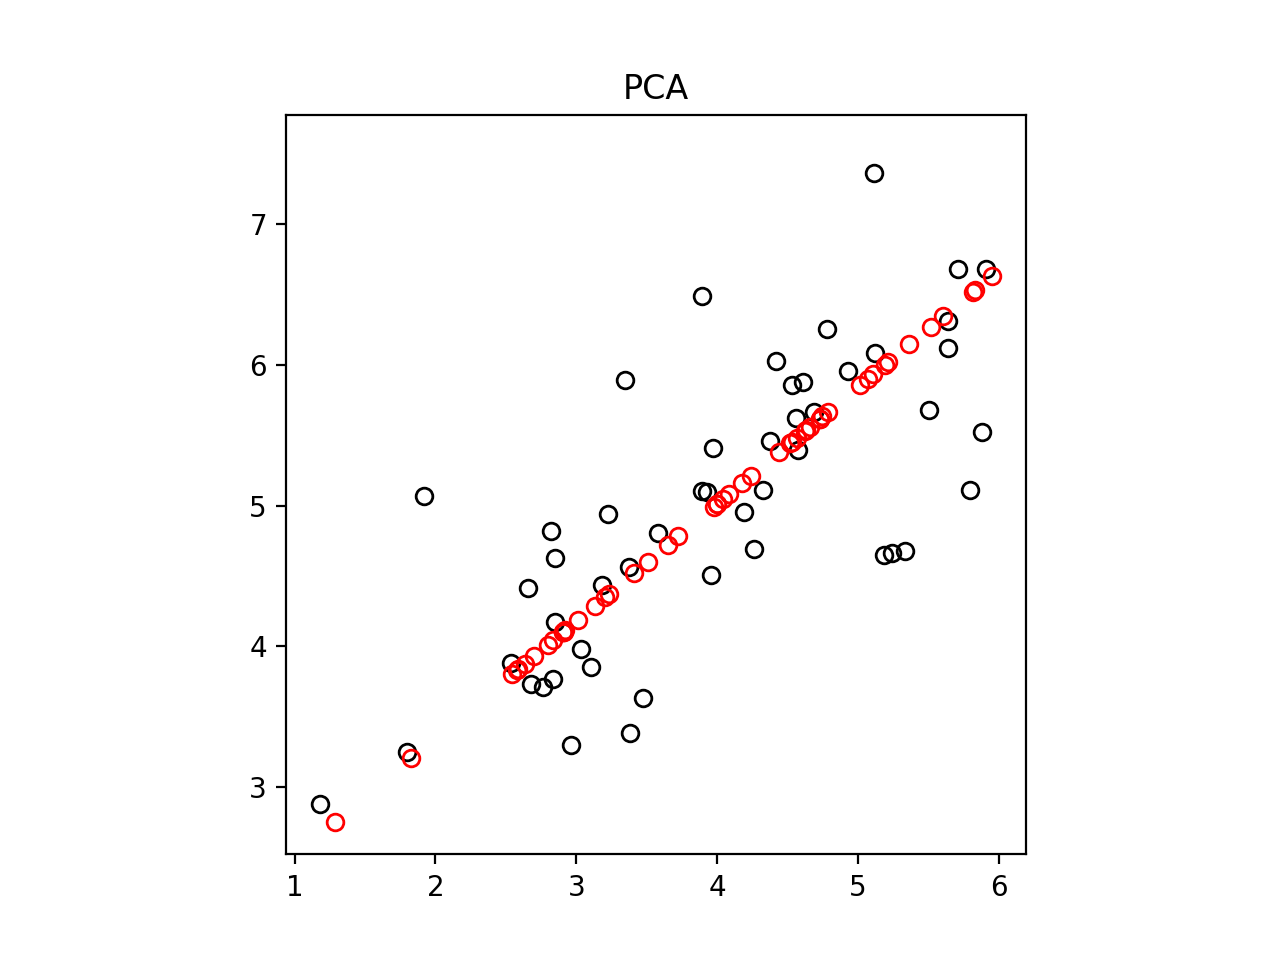
\includegraphics[width=0.5\linewidth]{figs/Chap_15_PCA.png}
\end{figure}

\begin{lstlisting}[language=Python]
"""
class sklearn.decomposition.PCA(n_components=None, *, copy=True, whiten=False, 
svd_solver='auto', tol=0.0, iterated_power='auto', random_state=None)
"""

import numpy as np
from scipy.io import loadmat
import matplotlib.pyplot as plt
import matplotlib
from sklearn.decomposition import PCA

X = loadmat('data/ex7faces.mat')['X']
X = np.transpose(X.reshape((5000, 32, 32)), [0, 2, 1]).reshape(5000, 1024)
X = -X

pca = PCA(n_components=0.99)
pca.fit(X)
redX = pca.transform(X) # reduced X
recX = pca.inverse_transform(redX) # recovered X

def show_a_face(face, ax):
	"""
	face.shape: (1024, )
	"""
	ax.matshow(face.reshape((32, 32)), cmap=matplotlib.cm.binary)
	ax.axis('off')

fig, ax = plt.subplots(5)
fig.suptitle('99% variance', fontweight='bold')
fig.subplots_adjust(hspace=0, wspace=None)
for i in range(5):
	show_a_face(recX[i], ax[i])
plt.show()
\end{lstlisting}

\begin{figure}[H]
    \centering
    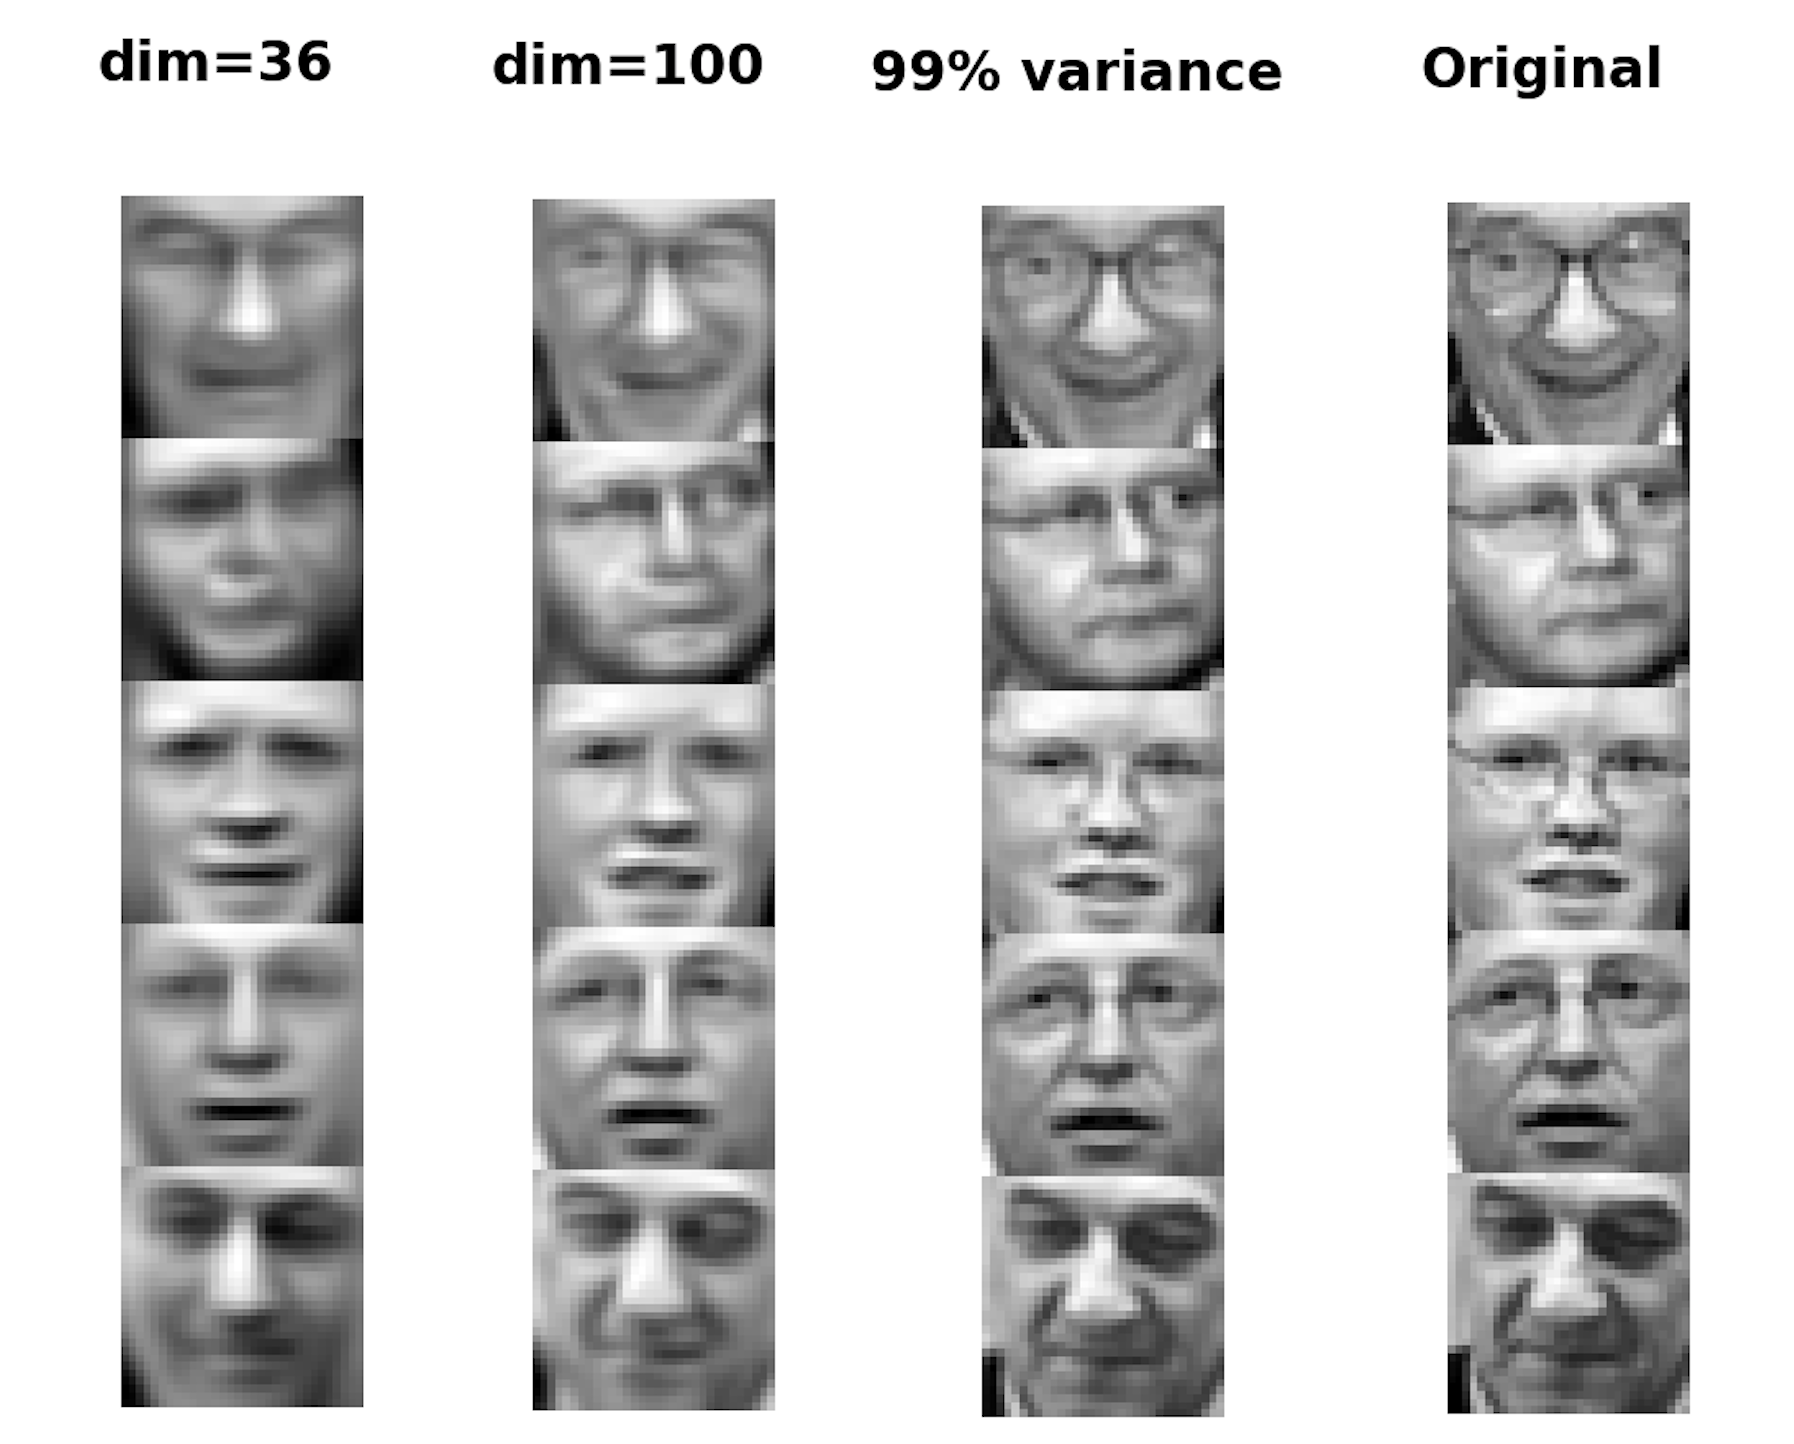
\includegraphics[width=0.5\linewidth]{figs/Chap_15_PCA2.png}
\end{figure}

\paragraph{异常检测}

\begin{center}
\begin{lstlisting}[language=Python]
"""
class sklearn.covariance.EllipticEnvelope(*, store_precision=True, assume_centered=False, 
support_fraction=None, contamination=0.1, random_state=None)

sklearn.metrics.f1_score(y_true, y_pred, *, labels=None, pos_label=1, 
average='binary', sample_weight=None, zero_division='warn')
"""

import numpy as np
from scipy.io import loadmat
from sklearn.covariance import EllipticEnvelope
from sklearn.metrics import f1_score
import matplotlib.pyplot as plt

data = loadmat('data/ex8data1.mat')
X, Xval, yval = data['X'], data['Xval'], data['yval'].flatten()

bestc, bestf1 = 0, 0
for c in np.linspace(0, 0.1, 100):
	ano = EllipticEnvelope(contamination=c)
	ano.fit(X)
	pred = ano.predict(X)
	pred[pred==1] = 0
	pred[pred==-1] = 1
	f1 = f1_score(yval, pred)
	if f1 > bestf1:
		bestc, bestf1 = c, f1

ano = EllipticEnvelope(contamination=bestc)
print(bestc)
ano.fit(X)
pred = ano.predict(X)

ax = plt.subplot(1, 1, 1)
ax.set_xlabel('Latency (ms)')
ax.set_ylabel('Throughput (mb/s)')
ax.plot(X[:, 0], X[:, 1], 'x', alpha=0.5, color='blue')
ax.plot(X[pred==-1][:, 0], X[pred==-1][:, 1], 'o', color='red', markerfacecolor='none', ms=10)
plt.show()
\end{lstlisting}
\end{center}

\begin{figure}[H]
    \centering
    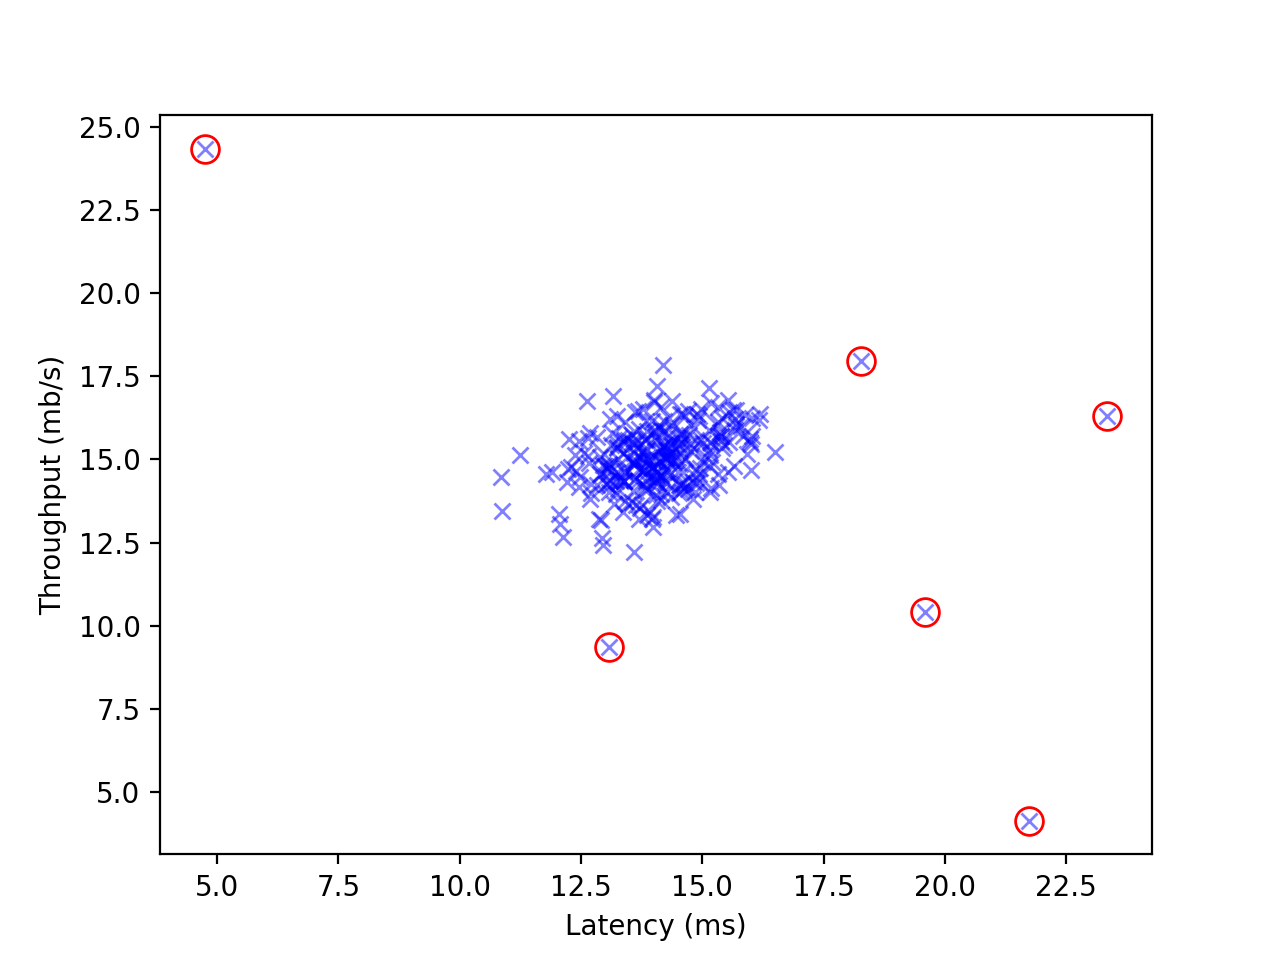
\includegraphics[width=0.5\linewidth]{figs/Chap_15_AnomalyDetection.png}
\end{figure}
